%###########################################################################
%
% Anhang
%
%###########################################################################
%\begin{appendix}
%\label{chap:Appendix}
%\chapter{Appendix A}
%\setcounter{chapter}{1}
%\addcontentsline{toc}{chapter}{Appendix}
%###########################################################################
% Anhang A
%###########################################################################
%\label{A}
%....


%\chapter{Appendix B}
%###########################################################################
% Anhang B
%###########################################################################
%\label{B}

%\pagebreak
%###########################################################################
%\end{appendix}


\renewcommand\thesection{\Alph{section}}
\renewcommand\thefigure{\thesection.\arabic{figure}}
\renewcommand{\thetable}{\thesection.\arabic{table}}
\setcounter{figure}{0}
\setcounter{table}{0}
\setcounter{section}{0}

\chapter*{Appendix}
\addcontentsline{toc}{chapter}{Appendix}

\label{chap:Appendix}

%-------------------------------------------------
\section{Electrical Power System} \label{sec:AppendixEPS}
%-------------------------------------------------
\begin{table}[htb]
\centering
\begin{tabular}{|c|c|}
\hline
\multicolumn{2}{|c|}{\textbf{SAFT 176065 xlr} \cite{SAFTBatteries.2018}}                                                                \\ \hline
\multicolumn{2}{|c|}{\textbf{Configuration:}}                                                                 \\ \hline
Battery Configuration                                                           & $4s3p$                        \\ \hline
Cells in Sereis $s$ N [-]                                                       & $4$                           \\ \hline
Cells in Parallel $p$ M [-]                                                     & $3$                           \\ \hline
\multicolumn{2}{|c|}{\textbf{Cell Parameters:}}                                                               \\ \hline
Typical Cell Capacity   [$Ah$]                                                    & $6.8$                         \\ \hline
Nominal Cell Voltage [$V$]                                                        & $3.65$                        \\ \hline
Nominal Cell Capacity [$Wh$]                                                      & $24.8$                        \\ \hline
Typical Cell Mass [$kg$]                                                          & $0.15$                        \\ \hline
Energy Density [$Wh/kg$]                                                     & $165.33$                      \\ \hline
\multicolumn{2}{|c|}{\textbf{Actual Battery Configuration Parameters:}}                                       \\ \hline
Battery Voltage $V_\text{Batt}$ [V]                                             & $14.6$                        \\ \hline
Battery Nominal Capacity $E_\text{Batt}$ [$Wh$]                                   & $297.6$                       \\ \hline
Battery Mass  [$kg$]                                                               & $1.8$                         \\ \hline
\textbf{Battery Mass} $m_\text{Batt}$ (incl. $10\%$ Margin) [$kg$]                                         & \textbf{1.98}                        \\ \hline
\multicolumn{2}{|c|}{\textbf{Configruation according to ECSS reliability restrictions and margins included:}} \\ \hline
Battery Configuration                                                           & $4s2p$                        \\ \hline
Cells in Sereis $s$ N [-]                                                       & $4$                           \\ \hline
Cells in Parallel $p$ M [-]                                                     & $2$                           \\ \hline
Battery Voltage $V_\text{Batt}$ [$V$]                                             & $14.6 $                       \\ \hline
Battery Nominal Capacity $E_\text{Batt}$ [$Wh$]                                   & $198.4$                       \\ \hline
$30\%$ Margin on Energy Content                                                 & $0.3$                         \\ \hline
\textbf{Battery Nominal Capacity} $E_\text{Batt}$ incl. Margin [$Wh$]                      & \textbf{138.88}                      \\ \hline
Useable Energy Density [$Wh/kg$]                                              & $70.14$                       \\ \hline
\end{tabular}
\caption{INSPIRE battery parameters.}
\label{tab:battery}
\end{table}

\begin{figure}[htb]
{\centering
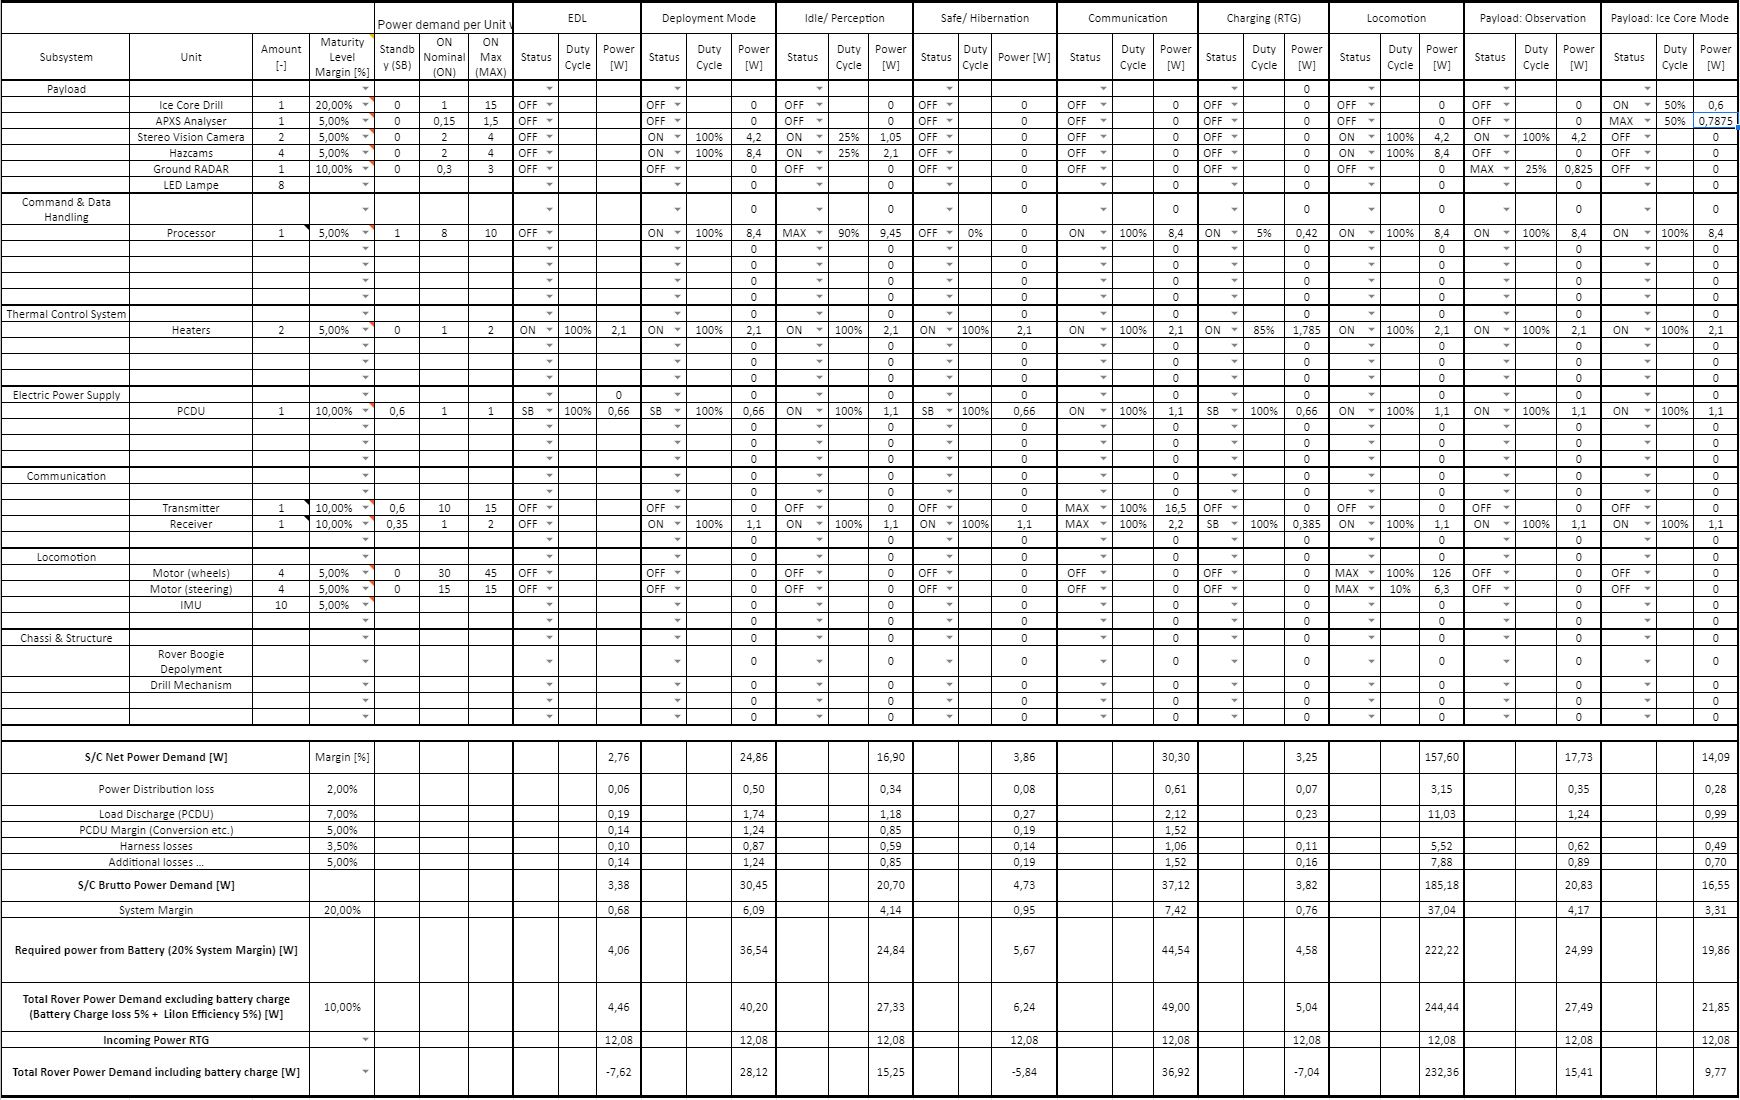
\includegraphics[width=1.0\textwidth]{Media/powerbudgetdummy}
\caption{POWER BUDGET DUMMY!}
\label{tab:powerbudgetcomplete}
}
\end{figure}

\clearpage
%-------------------------------------------------
\section{Thermal Controls System} \label{sec:AppendixThermal}
%-------------------------------------------------
\subsection{Heat energy eqilibrium}
The follwing equiations describe each node of the thermal network.
The input values were tanken from EPS or from \autoref{sec:app_therm_2}, \autoref{sec:app_therm_3}, \autoref{sec:app_therm_4}.\\

\underline{RTG:}
\[\dot{Q}_{RTG} +CON_1 \cdot (T_{Bay}-T_{RTG})+CON_2 \cdot (T_{Chassis}-T_{RTG})+CON_5 \cdot (T_{Drill}-T_{RTG})-\]
\[ - \epsilon_{RTG}\cdot \sigma_b \cdot S_{RTG}\cdot T_{RTG}^4= 0 \]\\


% CON \cdot (T_{}-T_{Node_2})
% CON \cdot (T_{}-T_{})
% \dot{Q}_{}
% \epsilon_{}\cdot \sigma_b \cdot S_{}\cdot T_{}^4

\underline{Electric Bay:}
\[ \dot{Q}_{Bay}+ CON_1 \cdot (T_{RTG}-T_{Bay})+ CON_3 \cdot (T_{Chas}-T_{Bay})  -\epsilon_{Bay}\cdot \sigma_b \cdot S_{Bay}\cdot T_{Bay}^4=0 \]
with: 
\[\dot{Q}_{B,intern} = \dot{Q}_{C\&DH} + \dot{Q}_{Tranceiver} +\dot{Q}_{Receiver} +\dot{Q}_{PCDU} \] \\

\underline{Drill \& Analyser:}
\[ \dot{Q}_{Drill} +CON_4 \cdot (T_{Chas}-T_{Drill})+CON_5 \cdot (T_{RTG}-T_{Drill}) = 0  \]\\

\underline{Camera:}
\[ \dot{Q}_{Cam} + \dot{Q}_{RHU} +CON_6 \cdot (T_{Chas}-T_{Cam})+(CON_{14} +n_{S1}\cdot CON_{S1}) \cdot (T_{Rad}-T_{Cam}) -\]
\[ - \epsilon_{Cam}\cdot \sigma_b \cdot S_{Cam}\cdot T_{Cam}^4= 0  \]\\

\underline{Radiator:}
\[  (CON_{14} +n_{S1}\cdot CON_{S1}) \cdot (T_{Cam}-T_{Rad}) - \epsilon_{Rad}\cdot \sigma_b \cdot S_{Rad}\cdot T_{Rad}^4= 0  \]\\

\underline{Chassis:}
\[ \dot{Q}_{Radar}+\dot{Q}_{Hazcam}  +CON_2 \cdot (T_{RTG}-T_{Chas})+CON_3 \cdot (T_{Bay}-T_{Chas})+\]

\[+CON_4 \cdot (T_{Drill}-T_{Chas})+ CON_6 \cdot (T_{Cam}-T_{Chas})+CON_7 \cdot (T_{Node_1}-T_{Chas}) +\]

\[ + \alpha_{Chas}\cdot [ q_{Sun} \cdot (1+\rho_E) \cdot (S_{Chas1} \cdot \varphi_1  +S_{Chas2} \cdot \varphi_2 ) +   \epsilon_{E} \cdot \sigma_b \cdot S_{Chas3}\cdot T_{Surface}^4 ]-\]

\[-\epsilon_{Chas}\cdot \sigma_b \cdot S_{Chas}\cdot T_{Chas}^4=0 \] \\[1em]


\underline{Steer Enine:}
\[ 4\cdot [\dot{Q}_{E,S} +(CON_8 +n_{S2}\cdot CON_{S2}) \cdot (T_{Node1}-T_{E,S})+CON_9 \cdot (T_{RTG}-T_{E,S}) -\epsilon_{E,S}\cdot \sigma_b \cdot S_{E,S}\cdot T_{E,S}^4]=0 \] \\


\underline{Distribution Node 1:}
\[ 4\cdot [CON_7 \cdot (T_{Chas}-T_{Node_1})+CON_8 \cdot (T_{E,S}-T_{Node_1})+CON_10 \cdot (T_{Node_2}-T_{Node_1})] = 0  \]\\

\underline{Drive Engine:}
\[ 4 \cdot [\dot{Q}_{E,D}+ (CON_{11}+n_{S3}\cdot CON_{S3}) \cdot (T_{Node_2}-T_{E,D})+ CON_{12} \cdot (T_{RTG}-T_{E,D})-\epsilon_{E,D}\cdot \sigma_b \cdot S_{E,D}\cdot T_{E,D}^4 ] = 0  \]\\

\underline{Distribution Node 2:}
\[ 4 \cdot [CON_{10} \cdot (T_{Node_1}-T_{Node_2})+CON_{11} \cdot (T_{E,D}-T_{Node_2})+CON_{13} \cdot (T_{Ground}-T_{Node_2})  ] = 0  \]\\


\subsection{Heat conductance} \label{sec:app_therm_2}

\subsection{Heat switch} \label{sec:app_therm_3}
The charateristic of the switch conductance depends on the mean temperature $T_M$, shown by measurements in cite .
As this temperature won´t be calculated in the analysis, the corresponding component temperature $T_C$ shall be used.
In order to describe the characteristic, it was diveded in three sections, \autoref{fig:tcs_switch03}.
The temperature where the disk decouples is $T_{toggle}=108 K$ and not applicable for the current application.
By reducing the heigt, the toggle temperature can be increased and the characteristic can be shifted to higher termperatures ("'to the right"').
It was assumed, that the gradients of section 2 and 3 as well as the temperature range of section 2 keep constant.
The axis interseption is a function the toggle temperature ($a_2=f(\Delta T_{toggle}),\ \Delta T_{Toggle}=T_{new}-T_{old}|_{toggle}$).

\begin{table}[H]
	\centering
	\begin{tabular}{c@{\qquad}rcl@{\qquad}l}
		\hline
		Section & \multicolumn{3}{l}{Temperature range} & Hear conductance $C_t= \frac{1}{R_t}$ \\ \hline
		1 & $T_{toggle} >$ & $ T_C  $ & & $C_{t,1}= 16.4 \cdot 10^{-3} \frac{W}{m^2 K} = const.$\\[1em]
		2 & $T_{toggle}\leq$ & $ T_C $ & $ < T_1$ & $C_{t,2} (T_C) = a_{1.1} \cdot T_C+ a_{1.2}$\\[1em]
		  & & & & $a_{1.1}= +1.272\cdot 10^{-3} \frac{W}{m^2 K^2}$ \\[1em]
		  & & & & $  a_{1.2}= -1.272\cdot 10^{-3} \frac{W}{m^2 K^2}\cdot \Delta T_{Toggle}-0.117 \frac{W}{m^2 K}$  \\[2em]
		3 & & 	$ T_C$ & $^ > T_1$ & $C_{t,3}(T_C) = a_{2.1} \cdot T_C+ a_{2.2}$\\[1em]
		& & & & $a_{2.1}=+ 333\cdot 10^{-6} \frac{W}{m^2 K^2}$ \\[1em]
		& & & & $  a_{2.2}= -333\cdot 10^{-6} \frac{W}{m^2 K^2}\cdot \Delta T_{Toggle}-28.3 \cdot 10^{-3} \frac{W}{m^2 K}$  \\[1em]\hline
	\end{tabular}
	\caption{Sections and range of the switch characteristic.}
	\label{tab:tcs_section}
\end{table}

\begin{figure}[H]
	\centering
	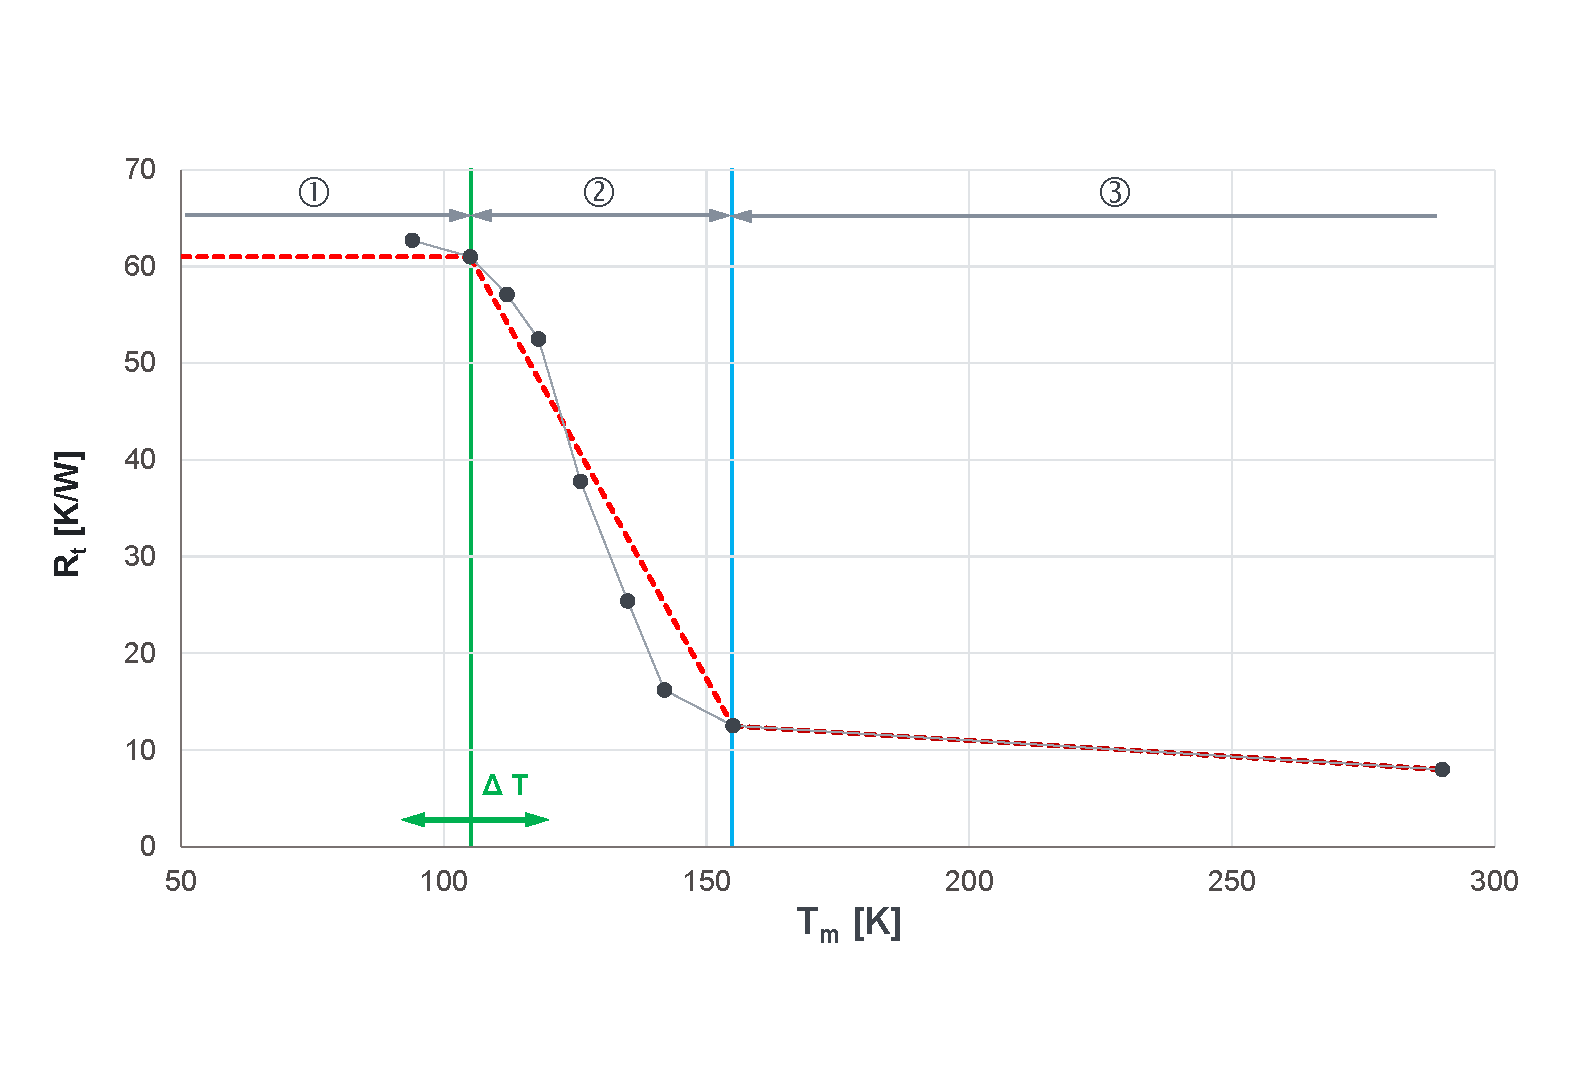
\includegraphics[width=1\textwidth]{Media/tcs_diag_section}
	\caption{Switch characteristic diveded in sections.}
	\label{fig:tcs_switch03}
\end{figure}

\subsection{Rover absorptivity} \label{sec:app_therm_4}
The amount of solar radiation onto the rover depends on the sun altitude, see autoref(fig:tcsabsop).

\begin{table}[H]
	\begin{tabular}{l@{\qquad}l}
		View Factor 1, Inclination:& $ \varphi_1=\cos (\lambda) \cdot \cos (\delta)  $ \\
		View Factor 2, Declination:&$ \varphi_2=\cos (90^{\circ}-\lambda) \cdot \cos (\delta)  $\\
	\end{tabular}
\end{table}





\subsection{Values} \label{sec:app_therm_5}
\begin{table}[htb]
	\centering
	\begin{tabular}{lcc}
		\hline
		 & \multicolumn{2}{l}{Temperature limits in [$^\circ C$]} \\ 
		Component	&	min. & max. \\\hline
		Command \& Data Handling & & \\
		Transmitter & -10 & 50 \\
		Receiver & -30 & 70 \\
		PCDU & -40 & 60 \\
		Battery & -35 & 60 \\
		Camera & -40 & 70 \\
		Objektive  & -40 & 71 \\
		Steering Engine & -30 & 100 \\
		Steering Gear & -30 & 85 \\
		Drive Engine & -40 & 100 \\
		Drive Gear & -40 & 100 \\ \hline
	\end{tabular}
	\caption{Temperatur limits of the rover components.}
	\label{tab:tcs_limits}
\end{table}

The Europas ground temperature varies at the  equator between $T_{e,min}=80K$ and $T_{e,max}=130 K$, depending on the sun inclination.
The temperature at the pole is $T_{Pole}=50K$, cite(europa).
It was assumed, that the ground temperature depends on the sun altitude.
A trigonometrical interpolation was defined as follows.
\[ T_{Ground}(\lambda, \delta) = T_{Pole} + \cos (\delta) \cdot [(T_{e,min}+\cos (\lambda)\cdot (T_{e,max}-T_{e,min}))-T_{Pole}] \]
For $\lambda$ and $\delta$ see \autoref{sec:app_therm_4}.


\begin{table}[htb]
	\centering
	\begin{tabular}{lccccc}
		\hline
		& \multicolumn{2}{l}{Emisivity [-]} & \multicolumn{2}{l}{Absorptivity [-]}& Source  \\ 
		Surface finishing	&	min. & max. 	&	min. & max.  & \\\hline
		Aluminium, polished & \multicolumn{2}{c}{0.045} & &  & \\
		Sand blasted alloy & & & & & \\
		White paint & & & & & \\
	\end{tabular}
	\caption{Minimum and maximum of surface emisivity and absorptivity values.}
	\label{tab:tcs_surface}
\end{table}




\begin{table}[htb]
	\centering
	\begin{tabular}{lccc}
		\hline
		Material & Nominal & Used & Source \\ \hline
		Aerogel & 0.002 - 0.05 & 0.05 & \\
		Aluminium & 236 & 236 & \\
		Copper$^{2)}$ &  400 & 360 & \\
		Steel$^{2)}$ & 21 - 50 & 21 & \\ \hline
		& & & \\
		\multicolumn{4}{l}{\small{$^{1)}$\ a reduction of 10\% was considered}}\\
		\multicolumn{4}{l}{\small{$^{2)}$\ depends on the alloying component, a conservative value was choosen }}\\
	\end{tabular}
	\caption{Heat conductivity in $\frac{W}{mK}$}
	\label{tab:tcs_conduct2}
\end{table}

\begin{table}[htb]
	\centering
	\begin{tabular}{lcc}
		\hline
		Part & Description & Value $m^2$  \\ \hline
		
	\end{tabular}
	\caption{Radiation surface of components.}
	\label{tab:tcs_surf}
\end{table}

%\begin{table}[H]
%	\centering
%	\begin{tabular}{llll}
%		\hline
%		Node & Description &  Connection & Suface  \\ \hline
%		RTG & & &   \\ 
%		Electric bay & & &   \\ 
%		Drill \& Analyser & & &   \\ 
%		Camera & & &   \\ 
%		Radiator & & &   \\ 
%		Chassis & & &   \\ 
%		Distributio Node 1 & & &   \\ 
%		Steering Engine & & &   \\ 
%		Distributio Node 2 & & &   \\
%		Drive Engine & & &   \\  
%	\end{tabular}
%	\caption{Description of thermal nodes.}
%	\label{tab:tcs_nodes}
%\end{table}

\clearpage

\section{Radiation}

\label{sec:AppendixRadiation}

In this chapter, detailed calculations are performed on which \autoref{sec:Radiation} is based on. All calculations and figures in \autoref{sec:AppendixRadiation} are performed with SPENVIS unless otherwise stated. In order to simulate the radiation on Europa an orbit around Jupiter is simulated with the orbit parameters of Europa with a total mission duration of 30 days. The chosen parameters were an perijove altitude of 664,862 km, an apojove altitude of 676,938 km, and an inclination of 0.47°.

\subsection{Jupiters Radiation Environment}

\label{subsec:AppendixRadiationEnvironment}

In order to compare the radiation environment around Jupiter and the radiation environment around Earth the following trapped radiation models were used: for Jupiter the D\&G83+Salammbo proton model and D\&G83+GIRE+SalammboE electron model was used; for Earth the AP-8 proton model and the AE-8 electron model was used.

\begin{figure}[htb]
     \centering
     \begin{subfigure}[b]{0.49\textwidth}
         \centering
         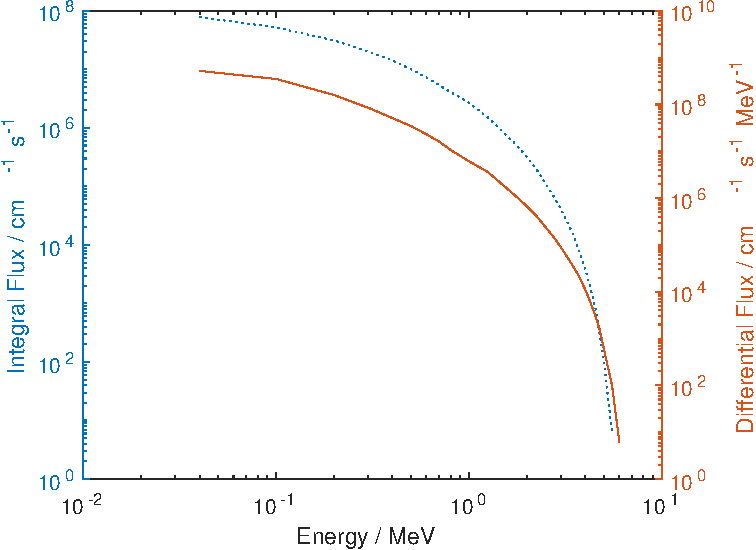
\includegraphics[width=\textwidth]{Media/E_Electron_Flux}
         \caption{Average spectra of trapped electrons around Earth}
         \label{fig:trappedelectronsEarth}
     \end{subfigure}
     \hfill
     \begin{subfigure}[b]{0.49\textwidth}
         \centering
         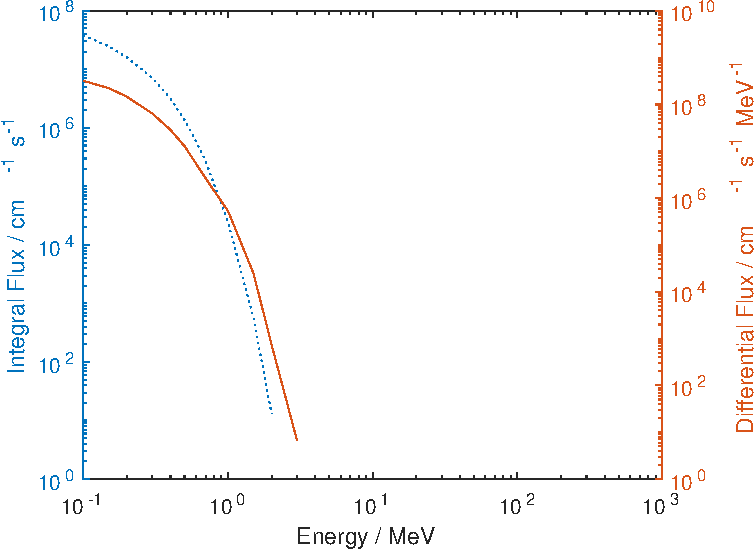
\includegraphics[width=\textwidth]{Media/E_Proton_Flux}
         \caption{Average spectra of trapped protons around Earth}
         \label{fig:trappedprotonsEarth}
     \end{subfigure}
     \hfill
     \begin{subfigure}[b]{0.49\textwidth}
         \centering
         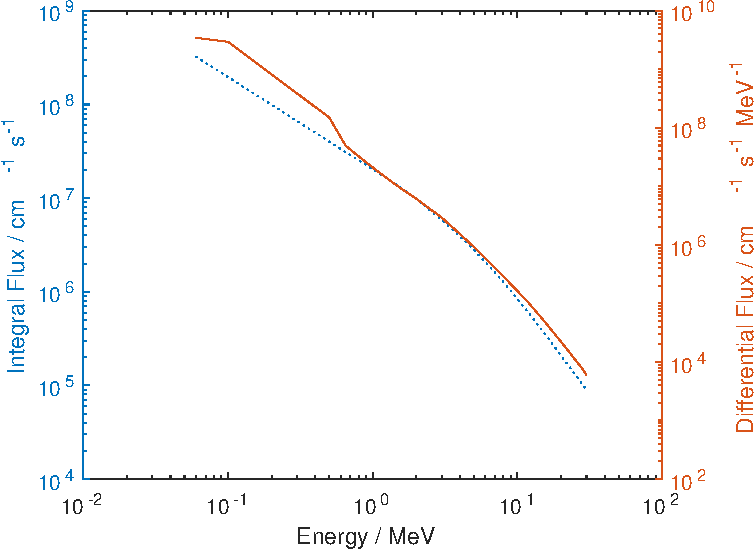
\includegraphics[width=\textwidth]{Media/J_Electron_Flux}
         \caption{Average spectra of trapped electrons around Jupiter}
         \label{fig:trappedelectronsJupiter}
     \end{subfigure}
     \hfill
     \begin{subfigure}[b]{0.49\textwidth}
         \centering
         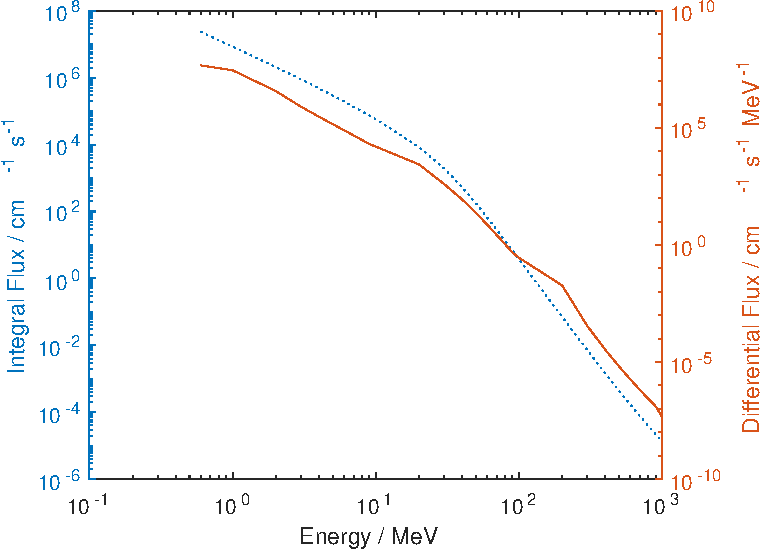
\includegraphics[width=\textwidth]{Media/J_Proton_Flux}
         \caption{Average spectra of trapped protons around Jupiter}
         \label{fig:trappedprotonsJupiter}
     \end{subfigure}
     \caption{Average trapped proton and electron fluxes on an orbit around earth at 25,000 km, through the outer Van Allen radiation belt, and on Europa's orbit around Jupiter.}
     \label{fig:trappedprotonelectronfluxes}
\end{figure}

\clearpage

\subsection{Radiation Exposures}

\label{subsec:AppendixRadiationExposures}

In order to simulate the TID for different radiation protections the Geant4 tool Multi-Layered Shielding Simulation (MULASSIS) is used. As target material silicon is selected with a thickness of 1 \(\mu \text{m}\). As shape a planar slap is selected because of the ice ground on one side of the rover.

\begin{figure}[htb]
     \centering
     \begin{subfigure}[b]{0.49\textwidth}
         \centering
         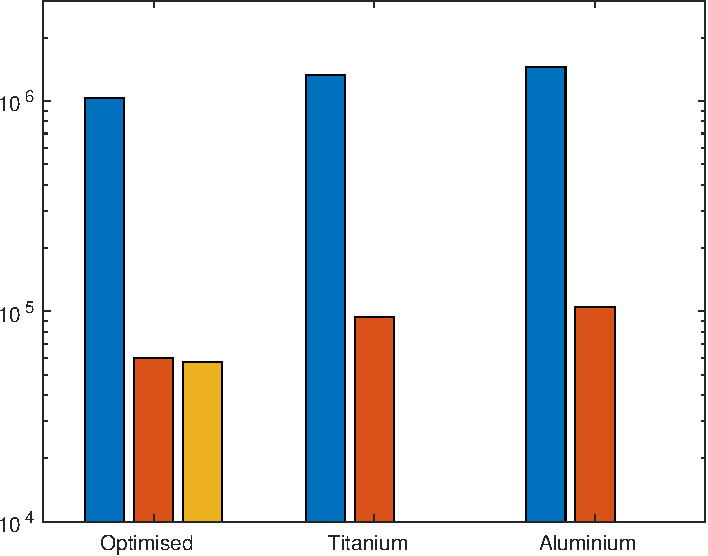
\includegraphics[width=\textwidth]{Media/J_Electron_Shielding}
         \caption{TID for Electrons as Source Particles}
         \label{fig:TIDElectronShielding}
     \end{subfigure}
     \hfill
     \begin{subfigure}[b]{0.49\textwidth}
         \centering
         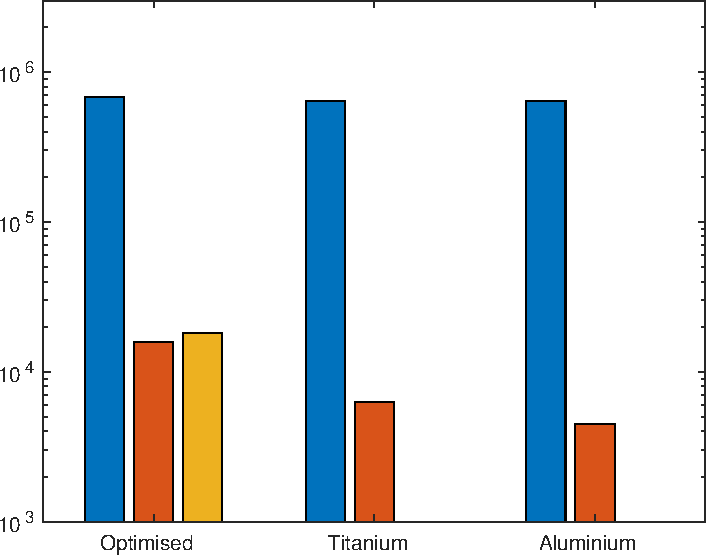
\includegraphics[width=\textwidth]{Media/J_Proton_Shielding}
         \caption{TID for Protons as Source Particles}
         \label{fig:TIDProtonShielding}
     \end{subfigure}
     \caption{TID of aluminium, titanium, and the optimised radiation structure shown in \autoref{tab:OptimalRadiationProtection} with a weight target of all three structures of 0.5 \(\text{g/cm}^2\) over 30 days of exposure on Europa.}
     \label{fig:AluminiumTitanOptimised}
\end{figure}

\begin{table}[htb]
\centering
\caption{Used components and the respective radiation tolerance and location}
\begin{adjustbox}{max width=\textwidth}
\begin{tabular}[l]{lccccc}

	\toprule
		Components	&	Rated TID	&	Exposed TID	&	Location\\
	\midrule
	
	Electric Motors	&	-	&	< 205 krad	&	locomotion housing\\	
	
	Harness	&	-	&	< 98 krad	&	chassis\\	
	
	Stereo Vision Cams	&	40	&	< 31 krad	&	camera housing\\	
	
	OBC	&	1000	&	< 17 krad	&	E-Bay\\
	
	PCDU	&	20	&	< 17 krad	&	E-Bay\\
	

	\bottomrule

\end{tabular}
\end{adjustbox}
\label{tab:RadiationList}
\end{table}

\begin{figure}[htb]
     \centering
     \begin{subfigure}[b]{0.49\textwidth}
         \centering
         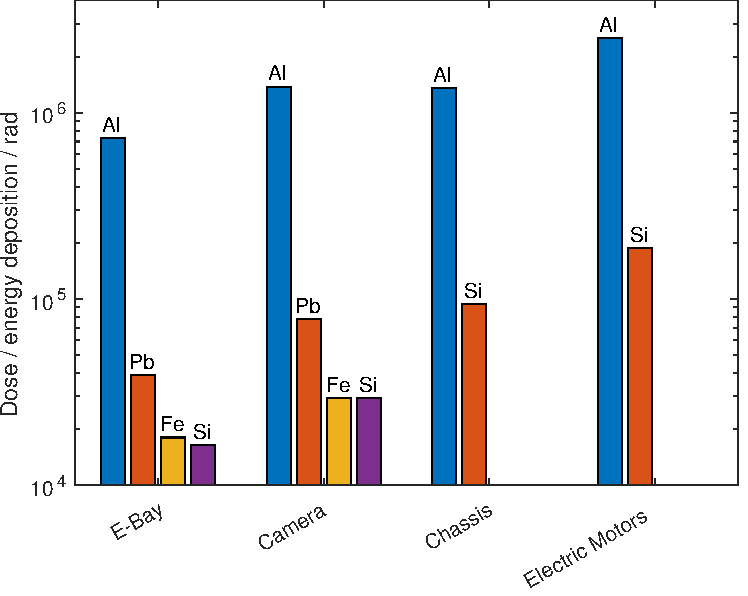
\includegraphics[width=\textwidth]{Media/J_Electron_Compartments}
         \caption{TID for Electrons as Source Particles}
         \label{fig:TIDElectronShielding}
     \end{subfigure}
     \hfill
     \begin{subfigure}[b]{0.49\textwidth}
         \centering
         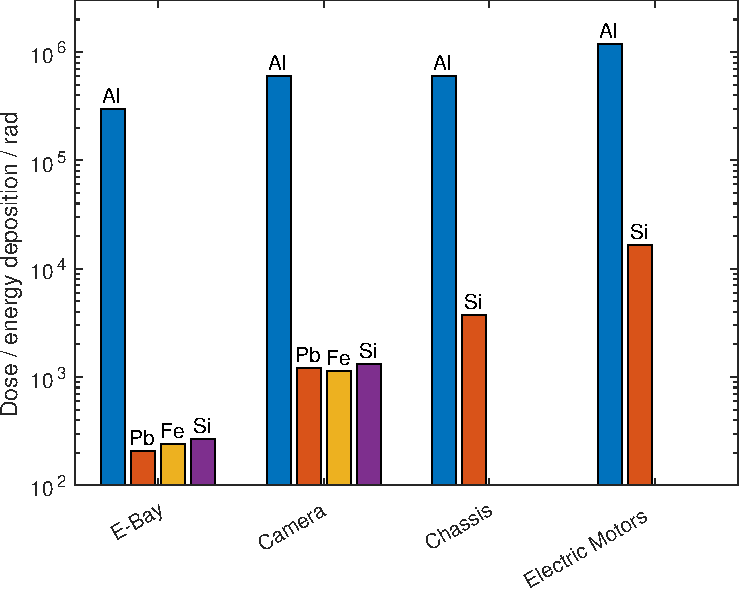
\includegraphics[width=\textwidth]{Media/J_Proton_Compartments}
         \caption{TID for Proton as Source Particles}
         \label{fig:TIDProtonShielding}
     \end{subfigure}
     \caption{TID for different compartments as seen in \autoref{fig:RadiationOverview}. The E-Bay is shielded by 4 mm aluminium, 0.415 mm lead, and 0.033 mm iron; the camera compartment by 2 mm aluminium, 0.415 mm lead, and 0.033 mm iron; the chassis by 2 mm aluminium; the electric motors by 1 mm aluminium.}
     \label{fig:CompartmentTID}
\end{figure}

\newpage

\subsection{Improvements}

\label{app:AppendixRadiationImprovements}

All simulations of the improvements introduced in \autoref{subsec:RadiationImprovements} are performed in the same way as in \autoref{subsec:AppendixRadiationExposures}. \\ \\
In \autoref{fig:Radiation_Improvements_Individual}, the TID over 30 days within the E-Bay is shown. If all components with an radiation resistance under 43.27 krad are shielded individually, the additional shielding structure around the E-Bay can be removed and the aluminium structure would be sufficient.

\begin{figure}[htp]
	\centering
	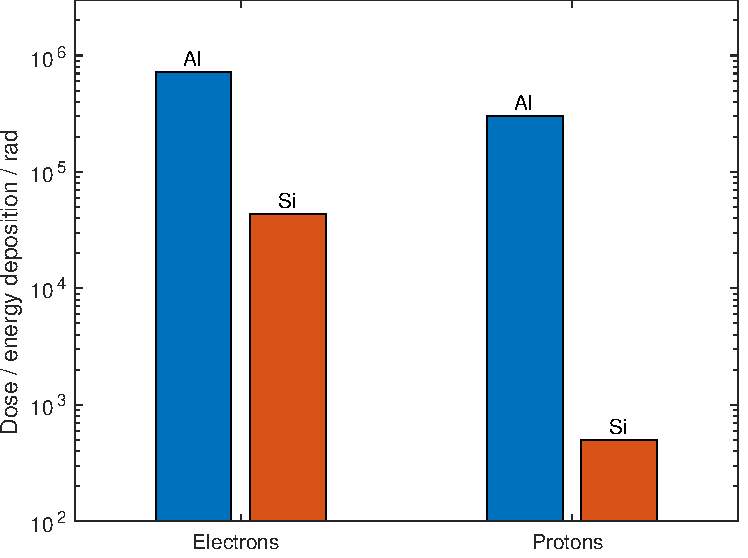
\includegraphics[width=0.7\textwidth]{Media/J_Improvements_Individual}
	\caption{TID with 4 mm Al shielding over a mission duration of 30 days}
	\label{fig:Radiation_Improvements_Individual}
\end{figure}

The resulting mass savings can be calculated with \autoref{eq:RadiationImprovementsIndividual} with \(m^*\) as the specific weight of the radiation protection and \(N\) as the amount of components within the E-Bay with a radiation resistance under 43.27 krad as of \autoref{tab:RadiationList}.

\begin{equation}
	\Delta m = SA_\text{E-Bay} \cdot m^*_\text{Shielding} - \sum\nolimits_{n=0}^N SA_\text{Component, n} \cdot m^*_\text{Shielding}
	\label{eq:RadiationImprovementsIndividual}
\end{equation}

With inserted values this results in a mass saving of \(\Delta m\) = 736.2 g.

\begin{figure}[htp]
	\centering
	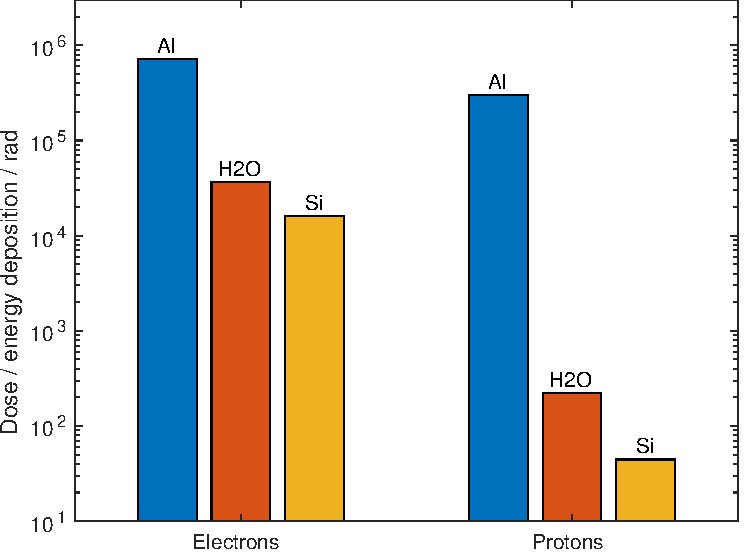
\includegraphics[width=0.7\textwidth]{Media/J_Improvements_Ice}
	\caption{TID with 4 mm Al shielding and 1 cm of Water over a mission duration of 30 days}
	\label{fig:Radiation_Improvements_Ice}
\end{figure}


\clearpage


%-------------------------------------------------
\section{Communications} 
\label{sec:AppendixCOM}
%-------------------------------------------------

\subsection{Link Budget}

Link budget considerations are performed under the conservative assumptions listed in \autoref{tab:lb-param}. \\

\begin{table}[]
\centering
\begin{tabular}{llclll}
\hline
Parameter                        & Value  & Unit	       & Symbol        & Source                       &  \\ \hline
Rover                            &        &            &               &                              &  \\ \hline\hline
antenna Gain           		     & 2      & {[}dB{]}   & ${G}_{R}$  	   & omnidirectional LGA          &  \\
output power        	         & 1      & {[}W{]}    & ${P}_{R}$  	   &                              &  \\
line loss               	     & 0,6    & {[}dB{]}   & ${L}_{l1}$ 	   & FLP                          &  \\ \hline
Path                             &        &            &               &                              &  \\ \hline\hline
R2L polarisation loss            & 0,3    & {[}dB{]}   & ${L}_{p}$ 	   & FLP                          &  \\
free space loss                  & 117,55 & {[}$m^3${]}& ${L}_{s}$  	   &                              &  \\
atmospheric loss                 & 0      & {[}dB{]}   & ${L}_{a}$	   & negligible atmosphere        &  \\ \hline
Lander                           &        &            &               &                              &  \\ \hline\hline
antenna Gain             		 & 1      & {[}dB{]}   & ${G}_{L}$	   & conservative estimation      &  \\
output power        	         & 5      & {[}W{]}    & ${P}_{L}$  	   & conservative estimation      &  \\
pointing Loss  		             & 0      & {[}dB{]}   & ${n/a}$       & omnidirectional LGA          &  \\
line Loss  		                 & 0,6    & {[}dB{]}   & ${L}_{l2}$	   & FLP                          &  \\
eff. noise temperature           & 300    & {[}K{]}    & ${T}_{s}$	   & worst case E-bay temperature &  \\ \hline
Demodulation \& Uncertain Losses &        &            &               &                              &  \\ \hline\hline
eff. data rate                   & 5000   & {[}kbps{]} & ${R}$         &                              &  \\
FEC coding                       & none   & {[}-{]}    & ${n/a}$       &                              &  \\
technical degradation            & 1      & {[}dB{]}   & ${L}_{i1}$    & FLP                          &  \\
implementation loss              & 1      & {[}dB{]}   & ${L}_{i1}$	   & FLP                          &  \\
                                 &        &            &               &                              & 
\end{tabular}
\caption{Rover to Lander (R2L) transmission parameters}
\label{tab:lb-param}
\end{table}

The free space loss ${L}_{s}$ [$m^3$] in \autoref{tab:lb-param} is calculated using the following correlation. 

\begin{equation}
\centering
	{L}_{s} = {\frac{(4 \pi s)^2 \cdot c}{f}}
\label{eqn:Ls}
\end{equation}

The signal travel distance {s} is assumed to be $s = 2\ km$ which is in excess of the mission goal. In accordance with X-Band communication the frequency {f} is set to a value of $f = 8,2\ GHz$. The parameter c represents the speed of light in vacuum. For simplification purposes $c = 3 \cdot 10^9\ \frac{m}{s}$ is assumed. \\ \\   
Combining the parameters from \label{tab:lb-param} the link budget is calculated using \autoref{eqn:EbzuN0}. For the simplification of \autoref{eqn:EbzuN0} the line losses for the rover ${L}_{l1}$ and lander ${L}_{l2}$ are expressed as the sum ${L}_{l}$. Technical degradation and implementation losses are combined to ${L}_{i}$ in the same manner.  

\begin{equation}
	\centering
		\frac{{E}_{b}}{{N}_{0}} = {P} - {L}_{l} + {G}_{R} - {10\cdot \log{{L}_{s}} - {L}_{a} + {G}_{L} + {10\cdot \log{k}} - {10\cdot \log{{T}_{s}}} - {10\cdot \log{{R}}} - {L}_{i}
	\label{eqn:EbzuN0}
\end{equation}

As can be seen in \label{tab:lb-param} the parameters 
\clearpage



%-------------------------------------------------
\section{Locomotion} 
\label{app:Loco}
%-------------------------------------------------

\subsection{Locomotion Design Drivers}
\label{app:DesignDrivers}

\begin{figure}[htb] 
  \centering
     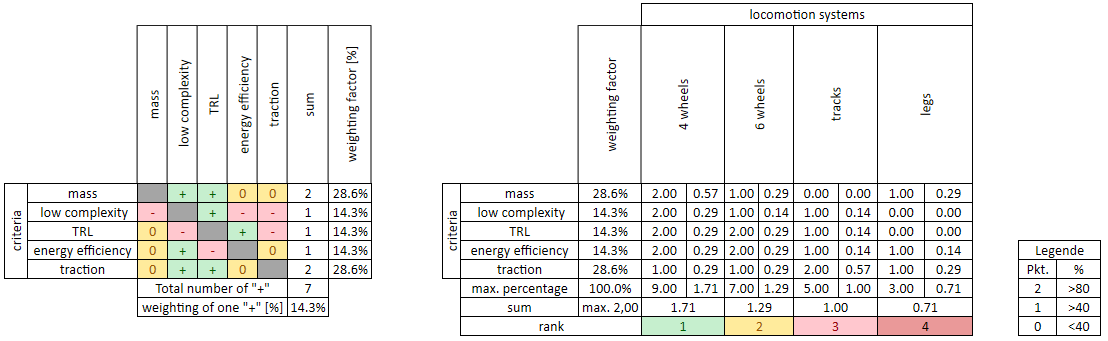
\includegraphics[width=1\textwidth]{Media/LocomotionTradeOff.png}
  \caption{Trade-off of the locomotion movement system. The criteria with the respective weighting factors are shown on the left. On the right side are the respective systems.}
  \label{fig:TradeOffLoco}
\end{figure}


\begin{figure}[htb] 
  \centering
     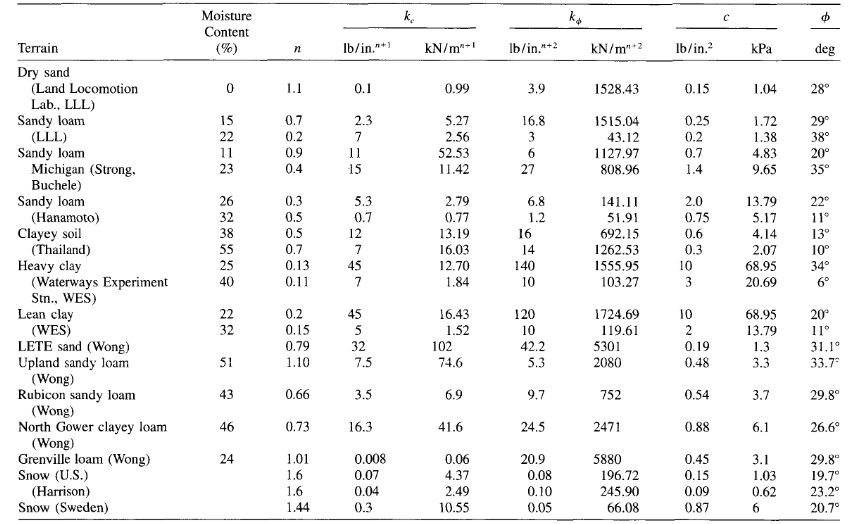
\includegraphics[width=1\textwidth]{Media/SoilParameters.png}
  \caption{Soil Parameters}
  \label{fig:SoilParameters}
\end{figure}


\begin{figure}[htb] 
  \centering
     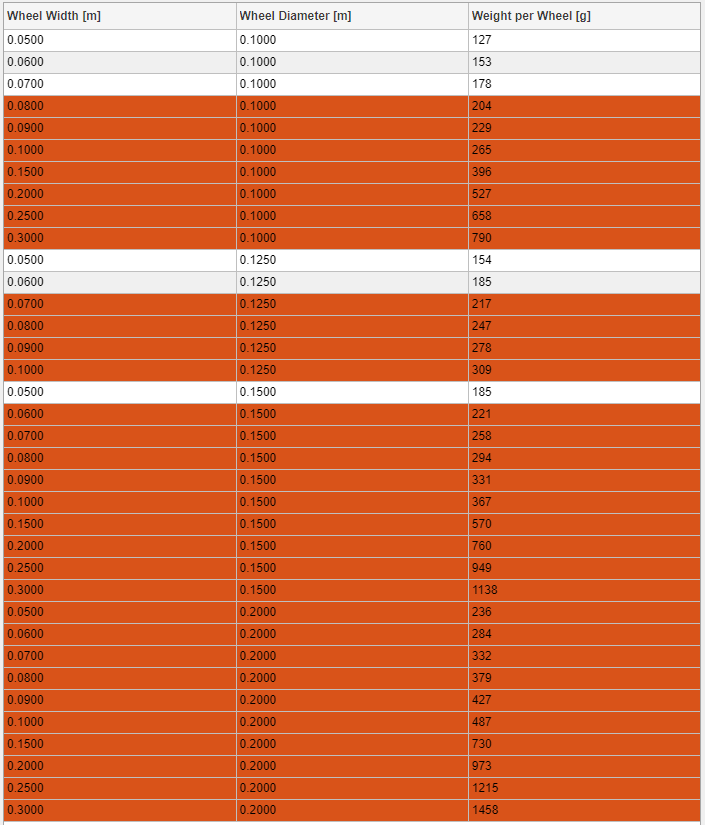
\includegraphics[width=1\textwidth]{Media/Dimensions-WeightLimits.png}
  \caption{Various wheel dimensions respective to the weight. Rows highlighted in red are not considered further for system design due to the limit of 200 g weight per wheel.}
  \label{fig:DimensionsLoco}
\end{figure}

\subsection{Formulas for Locomotion Parameters}
\label{app:FormulasLoco}


















\cleardoublepage

